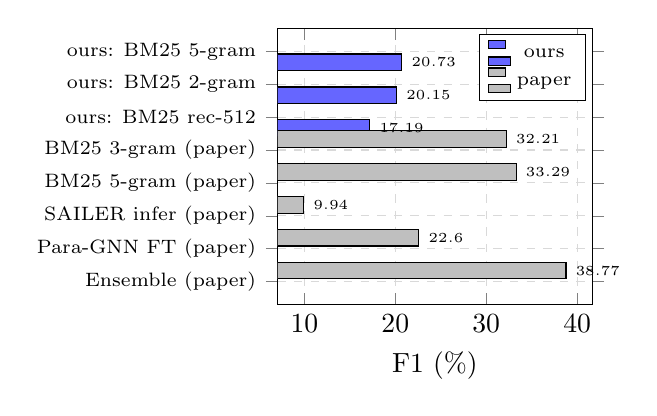
\begin{tikzpicture}
\begin{axis}[xbar, width=0.46\linewidth, height=0.42\linewidth,
  xlabel={F1 (\%)}, bar width=6pt,
  legend style={font=\scriptsize},
  nodes near coords, every node near coord/.append style={font=\tiny},
  ytick={0,1,2,3,4,5,6,7}, yticklabels={ours: BM25 5-gram,ours: BM25 2-gram,ours: BM25 rec-512,BM25 3-gram (paper),BM25 5-gram (paper),SAILER infer (paper),Para-GNN FT (paper),Ensemble (paper)},
  yticklabel style={font=\scriptsize}, y dir=reverse,
  grid=both, grid style={dashed,gray!30}]
\addplot[fill=blue!60] coordinates {(20.73,0) (20.15,1) (17.19,2)};
\addlegendentry{ours}
\addplot[fill=gray!50] coordinates {(32.21,3) (33.29,4) (9.94,5) (22.60,6) (38.77,7)};
\addlegendentry{paper}
\end{axis}
\end{tikzpicture}
